\documentclass[12pt]{report}

\usepackage{fullpage}
\usepackage{amsmath,amssymb,bm,upgreek,mathrsfs}
\usepackage{algorithmic,algorithm}
\usepackage{graphicx,subcaption}
\usepackage{setspace}
\usepackage{color}
\usepackage{multirow}
\usepackage{alltt}
\usepackage{cancel}
\usepackage{listings}

\doublespacing

\DeclareMathOperator*{\argmax}{arg\,max}
\DeclareMathOperator*{\argmin}{arg\,min}

\newcommand{\N}{\mathcal{N}} \newcommand{\U}{\mathcal{U}}
\newcommand{\Poi}{{\text Poisson}} \newcommand{\Exp}{{\text Exp}}
\newcommand{\G}{\mathcal{G}} \newcommand{\Ber}{{\text Bern}}
\newcommand{\Lap}{{\text Laplace}} \newcommand{\btheta}{\boldsymbol{\theta}}
\newcommand{\bSigma}{\boldsymbol{\Sigma}}

\newcommand{\E}[1]{\mathbb{E}[#1]}
\newcommand{\Cov}[2]{\mathbb{C}\mathrm{ov}(#1,#2)}

\def\*#1{\mathbf{#1}} \newcommand*{\V}[1]{\mathbf{#1}}

%%%%%%%%%%%%%%%%%%%%%%%%%%%%%%%%%%%%%%%%%%%%%%%%%%%%%%%%%%%%%%%%%%%%%%

\begin{document}

\centerline{\it CS 477} \centerline{\it HW \#3}

\centerline {Questions completed: All undergrad level questions and question B2}
\centerline {Programming/Deliverables: MATLAB} \centerline {Estimated time for
  assignment: 14 hours}

\begin{enumerate}
  
\item[A1.] Best fit line using least squares
  
  Below in Figure 1, I provide the plot of the two best fit lines of the data
  points from line\_data\_2.txt using non-homogenous and homogenous least
  squares as covered in class.
  \newpage
  \begin{figure}[h!]
    \centering \fbox{\begin{minipage}{.98\linewidth}
        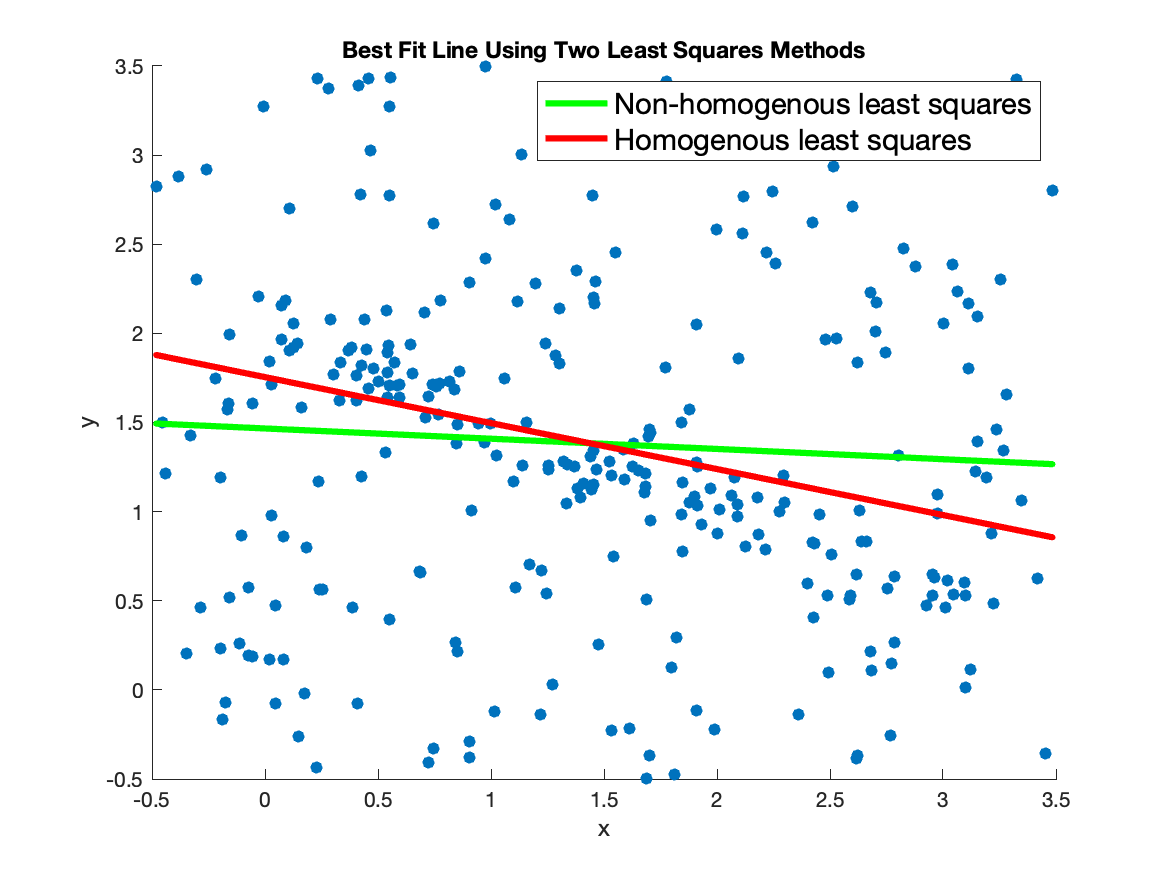
\includegraphics[width=\linewidth]{a1.png}
        \caption{The blue dots are the data points from line\_data\_2.txt. The
          green line is the best fit line using non-homogenous least squares
          which fits the line based on vertical distance to all the points. The
          red line is the best fit line using homogenous least squares which
          fits the line based on perpendicular distance to all the points.}
        \label{fig:a1}
    \end{minipage}}
  \end{figure}
  The non-homogenous least squares best fit line (green line in Figure 1) was
  calculated by rewriting the slope-intercept equation of a line $y=mx+b$ as $(x
  1)*(m ; b)=y$ where U is a matrix with rows $(x_i\ 1)$ (a column with the x
  vector and another column of 1s), y is the vector of $y_i$ elements, and $x=(m
  ; b)$ is a vector unknowns. The equation thus becomes $Ux=y$ and in MATLAB we
  can solve this by doing $x=U \setminus y$ to get our slope m and intercept b.
  
  The homogenous least squares best fit line (red line in Figure 1) was calculated
  by finding a line of the form $ax+by=d$. This was done by defining U as a
  matrix with rows $(x_i - \bar{x},\ y_i - \bar{y})$ and defining $Un=0$ where
  vector $n=(a,\ b)$ and $a^2+b^2=1$. Given $Y=U'*U$ and using $eig(Y)$ in
  MATLAB returns a 2x2 matrix of eigenvectors and another 2x2 matrix of
  eigenvalues.  The column with the minimum eigenvalue corresponds to the column
  with the eigenvector we are looking for, and it happened to be the first
  column in our case. Thus, that was the answer to our vector n and now constant
  d can be computed with $d=a\bar{x} + b\bar{y}$.  Finally, we have our line
  $ax+by=d$ which is rewritten as $y = -ax/b + d/b$ to plot on our graph.
  
  Visually speaking, in Figure 1, homogenous least squares seems to produce the
  'better' line when eyeballing the data and seeing that it aligns closer to the
  cluster of points in the middle. When working with data in line\_data.txt
  which had little noise, the lines produced from both methods were almost
  overlapping, but it can observed here that perhaps homogenous least squares
  works better when there is more noise in the data.
  
  \newpage
  I provide the required stats for both best fit lines below in Figure 2.
  
  \begin{figure}[h!]
    \centering
    \fbox{\begin{minipage}{.98\linewidth}
        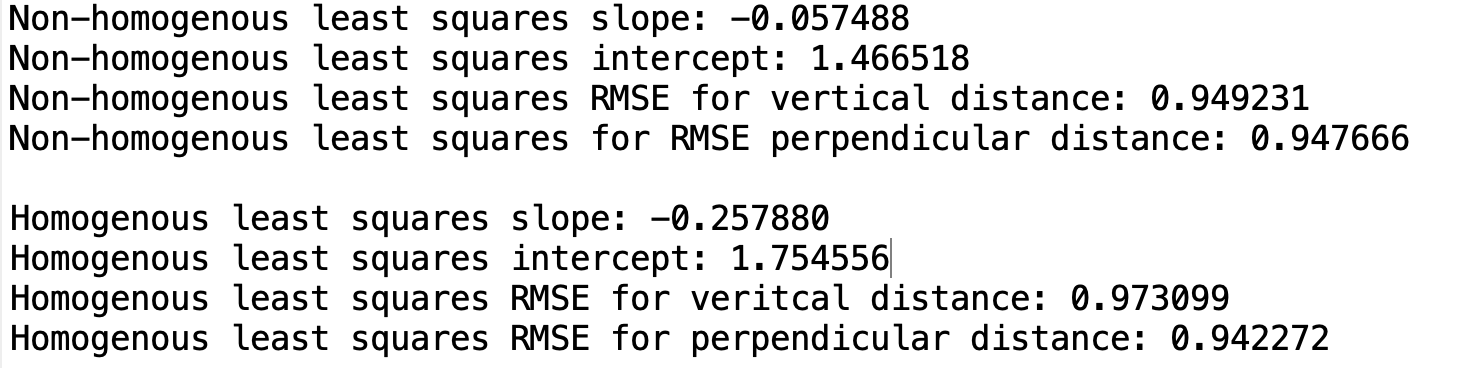
\includegraphics[width=\linewidth]{a1b.png}
        \caption{Calculations and output were generated in MATLAB. }
        \label{fig:a1b}
    \end{minipage}}
  \end{figure}
  In Figure 2, the slopes and intercepts of the best fit lines were already
  computed previously when we were trying to plot them on the graph. Comparing
  the slopes of non-homogenous versus homogenous least squares in Figure 2, we
  can see that they are consistent with the plots in Figure 1. The
  non-homogenous slope is close to zero and we can see correspondingly that the
  non-homogenous (green) line in Figure 1 is close to horizontal in nature. The
  homogenous (red in Figure 1) slope on the other hand is more negative and we
  can see in Figure 1 that it is angled more downwards. Similarly, we can see
  that the intercepts for both best fit lines are consistent with what we see in
  Figure 1.
  
  For calculating the root mean sqaure error (RMSE) with respect to (w.r.t.)
  vertical distance, we take the difference between the y values on the best fit
  line and actual y values of the points (at every x value) and go on to take
  the RMSE of the differences. This was done for both non-homogenous and
  homogenous error in Figure 2.
  
  For calculating the RMSE w.r.t. to the perpendicular distance between points,
  we first compute the perpendicular distance between points to the the best fit
  line.  For the homogenous line, the perpendicular distance is given by $ax +
  bx - d$ which we already have from computing the line, so we get this for
  free. For our non-homogenous line of the form $y=mx+b$, we can rewrite it as
  $mx-y+b=0$ where $a=m, b=-1, d=-b$ (referring to $ax+by=d$, not to get
  confused with the b's) and compute its perpendicular distance to every point
  given by $distance=\frac{ax+bx-d}{\sqrt(a^2+b^2)}$. With the perpendicular
  distances computed, we can the RMSE of the differences as usual for both
  non-homogenous and homogenous lines, and they are also reported in Figure 2.
  
  Looking at the RMSEs in Figure 2, we can see that the non-homogenous error is
  lower than the homogenous error w.r.t. vertical distance. This is consistent
  with what we expect because the non-homogenous line is fitted w.r.t. to the
  vertical distance while the homogenous line is fitted w.r.t. to the
  perpendicular distance. We can also see in Figure 2 that the homogenous error
  is lower than the non-homogenous error w.r.t. to perpendicular distance,
  albeit very slightly. This is consistent with we expect because homogenous
  least square fits the line w.r.t. to perpendicular distance between
  points. However, the fact that the perpendicular RMSEs are so close in value
  despite the lines coming from two different models and being clearly distinct
  in Figure 1 raises uncertainty in my results. It could be that my computations
  were off for perpendicular RMSE for the non-homogenous and/or homogenous
  lines. It could also be that the small optimization in perpendicular RMSE from
  the non-homogenous (red) line to homogenous (green) line in Figure 1 is enough
  to produce the distinguishable result in best fit lines.
  
  
  Interestingly, in Figure 2, the non-homogenous RMSE w.r.t. the perpendicular
  distance is slightly lower than its RMSE w.r.t. vertical distance despite the
  fact that non-homogenous least squares uses vertical distance. My explanation
  for this observation is that, first, since the non-homogenous best fit line is
  close to zero and thus lies almost horizontal on the graph, its perpendicular
  and its vertical distance to the points must be close in value to each
  other. With this fact in mind, it could be a coincidence that the
  non-homogenous perpendicular RMSE is slightly lower than its vertical
  RMSE. Another explanation is a computational error on my part that
  misrepresents the non-homogenous and/or homogenous perpendicular RMSE. I would
  have expected homogenous perpendicular RMSE to be lower than the report in
  Figure 2 based on the better fitting of the homogenous line visually in Figure
  1.
  
\item[B1.] Visually determining a perspective image
  
  I provide the analyzed building.jpeg image below in Figure 3.
  \begin{figure}[h!]
    \centering
    \fbox{\begin{minipage}{.98\linewidth}
        \includegraphics[width=\linewidth]{Screenshot 2024-09-22 at 11.33.01 PM.png}
        \caption{Parallel lines were drawn for building.jpeg to look for
          vanishing points of parallel lines as well as the colinearity of
          vanishing points of parallel lines on the same plane.}
        \label{fig:building}
    \end{minipage}}
  \end{figure}
  
  In Figure 3, a clear vanishing point can be seen for the vertical lines of the
  main buliding shown by the pink lines. Off to the top right of Figure 3, black
  lines are drawn for two buildings, and two black lines for one building can be
  seen reaching the same vanishing point of the main buliding while the other
  building has two black lines reaching a slightly lower vanishing point. So
  far, the property of parallel lines converging to a vanishing point is
  present, but the property of vanishing points on the same plane being colinear
  is unclear.
  
  Looking at the green and light blue lines in Figure 3 which are on the same
  plane as the pink lines, it seems that the green lines lead to a vanishing
  point far off the screen, and the light blue lines, created by going 6 floors
  up and across the building, seem to be literally parallel with each other and
  not leading to a vanishing point any time soon. Thus, it can be concluded that
  the vanishing points on the same plane are not colinear, if at all even there
  with the light blue lines.
  
  Thus, this image as shown in Figure 3 is not in perspective. My additional
  thoughts on this image is that it is AI enhanced or AI generated. On closer
  inspection, one can see that the height of the floors are not consistent, and
  the floor around where the highest blue line meets the right corner of the
  building is much taller than the other floors in particular which does not
  make sense. Other observations in Figure 3 are the piece of buliding on the
  top left corner of the image which seems to random, and what are supposed to
  be the reflections of (hovering? or impossibly tall?) lamp posts near the
  bottom of the building do not make sense when scrutinized.
  
  \newpage
\item[B2.] Visually determining a perspective image part 2
  
  I provide the image of chandelier.tiff in Figure 4 below.
  \begin{figure}[h!]
    \centering
    \fbox{\begin{minipage}{.98\linewidth}
        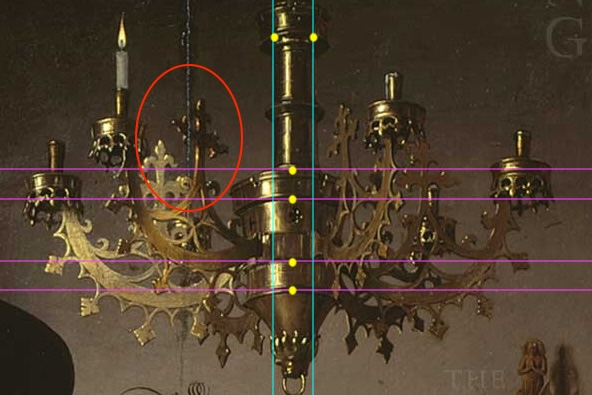
\includegraphics[width=\linewidth]{chandelier.jpeg}
        \caption{Parallel reference lines are drawn for chandelier.jpeg along
          its contours that are roughly parallel as color coded. The yellow
          circles indicate where the lines started. The red circle identifies a
          point of interest discussed below.}
        \label{fig:chandelier}
    \end{minipage}}
  \end{figure}
  
  In Figure 4, we start with the assumption that the image is perfectly
  symmetrical and draw some lines along obvious parallel parts of the
  chandelier. No obvious vanishing points are observed and upon inspection, we
  can see that the chandelier is not symmetrical at all, both with the main body
  and its arms. The asymmetry of the chandelier can be seen in its pointed
  ending at the bottom compared to the vertical blue lines which does not center
  evenly between them when observed closely in sections. The horizontal pink
  lines also reveal the asymmetry of chandelier's arms when comparing their
  mismatched elevations compared to the pink lines as well as their mismatched
  distance from the body of the chandelier. The red cirle in Figure 4 also
  brings to attention what is seemingly a rod that weaves in-between the
  cross-like metal on the top of one of the chandelier's arms which is
  impossible physically speaking, assuming that the metal cross is not warped,
  but on a straight plane as the image would suggest. Therefore, it can be
  concluded that the image is not symmetrical and is not a perspective
  image. Most likely, this image is AI-enhanced or AI generated.
\end{enumerate}

\end{document}
